\section{Ćwiczenia 5: 23-III-2017}

\subsection{Zadania Domowe A}
\paragraph{A1} Czy dla zaprezentowanych grafów prawdziwe jest podane oszacowanie na $\mathtt{MAX CUT}$?

Ogólna zasada:
\begin{itemize}
\item[$\rightarrow$] \textbf{RYSUNEK} oszacowanie z \textbf{DOŁU}
\item[$\rightarrow$] \textbf{WZÓR} oszacowanie z \textbf{GÓRY}
\end{itemize}

\begin{minipage}{.3\textwidth}
\begin{figure}[H]
\centering
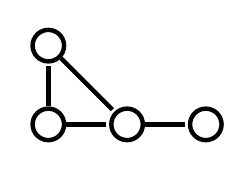
\begin{tikzpicture}[shorten >=1pt, auto, node distance=3cm, ultra thick,main node/.style={circle,draw,minimum size=.4cm,inner sep=0pt]}]%fill=black,
\begin{scope}[every node/.style={font=\sffamily\Large\bfseries}]
\node[main node] (v1) at (0,0) {};%1
\node[main node] (v2) at (0,1) {};%2
\node[main node] (v3) at (1,0) {};%3
\node[main node] (v4) at (2,0) {};%4
%\node[main node] (v) at (,) {};
\end{scope}
\begin{scope}[every edge/.style={draw=black,ultra thick}]
\draw  (v1) edge node{} (v2);
\draw  (v1) edge node{} (v3);
\draw  (v2) edge node{} (v3);
\draw  (v3) edge node{} (v4);
%\draw  (v) edge node{} (v);
\end{scope}
\end{tikzpicture}
\caption*{Oryginał: $\mathtt{MAX CUT}\leq 3$}
\end{figure}
\end{minipage}%
\begin{minipage}{.3\textwidth}
\begin{figure}[H]
\centering
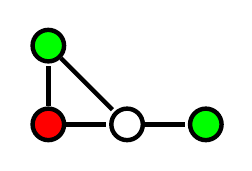
\begin{tikzpicture}[shorten >=1pt, auto, node distance=3cm, ultra thick,main node/.style={circle,draw,minimum size=.4cm,inner sep=0pt]}]%fill=black,
\begin{scope}[every node/.style={font=\sffamily\Large\bfseries}]
\node[main node,fill=red] (v1) at (0,0) {};%1
\node[main node,fill=green] (v2) at (0,1) {};%2
\node[main node] (v3) at (1,0) {};%3
\node[main node,fill=green] (v4) at (2,0) {};%4
%\node[main node] (v) at (,) {};
\end{scope}
\begin{scope}[every edge/.style={draw=black,ultra thick}]
\draw  (v1) edge node{} (v2);
\draw  (v1) edge node{} (v3);
\draw  (v2) edge node{} (v3);
\draw  (v3) edge node{} (v4);
%\draw  (v) edge node{} (v);
\end{scope}
\end{tikzpicture}
\end{figure}
\end{minipage}%
\begin{minipage}{.39\textwidth}
Wierzchołek bez koloru ma $3$ połączenia między wierzchołkami ,,kolorowymi'' $\Rightarrow \mathtt{MAXCUT}= 3$.
\end{minipage}

\begin{minipage}{.32\textwidth}
\begin{figure}[H]
\centering
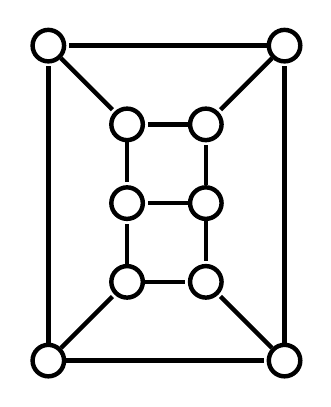
\begin{tikzpicture}[shorten >=1pt, auto, node distance=3cm, ultra thick,main node/.style={circle,draw,minimum size=.4cm,inner sep=0pt]}]%fill=black,
\begin{scope}[every node/.style={font=\sffamily\Large\bfseries}]
\node[main node] (v1) at (0,0) {};%1
\node[main node] (v2) at (3,0) {};%2
\node[main node] (v3) at (3,4) {};%3
\node[main node] (v4) at (0,4) {};%4
\node[main node] (v5) at (1,1) {};%5
\node[main node] (v6) at (2,1) {};%6
\node[main node] (v7) at (2,2) {};%7
\node[main node] (v8) at (2,3) {};%8
\node[main node] (v9) at (1,3) {};%9
\node[main node] (v10) at (1,2) {};%10
%\node[main node] (v) at (,) {};
\end{scope}
\begin{scope}[every edge/.style={draw=black,ultra thick}]
\draw  (v1) edge node{} (v2);
\draw  (v1) edge node{} (v4);
\draw  (v1) edge node{} (v5);
\draw  (v2) edge node{} (v3);
\draw  (v2) edge node{} (v6);
\draw  (v3) edge node{} (v4);
\draw  (v3) edge node{} (v8);
\draw  (v4) edge node{} (v9);
\draw  (v5) edge node{} (v6);
\draw  (v5) edge node{} (v10);
\draw  (v7) edge node{} (v6);
\draw  (v7) edge node{} (v8);
\draw  (v7) edge node{} (v10);
\draw  (v8) edge node{} (v9);
\draw  (v9) edge node{} (v10);
%\draw  (v) edge node{} (v);
\end{scope}
\end{tikzpicture}
\caption*{$\mathtt{MAX CUT} \geq 4$}
\end{figure}
\end{minipage}%
\begin{minipage}{.32\textwidth}
\begin{figure}[H]
\centering
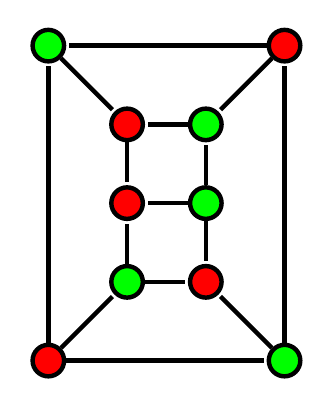
\begin{tikzpicture}[shorten >=1pt, auto, node distance=3cm, ultra thick,main node/.style={circle,draw,minimum size=.4cm,inner sep=0pt]}]%fill=black,
\begin{scope}[every node/.style={font=\sffamily\Large\bfseries}]
\node[main node,fill=red] (v1) at (0,0) {};%1
\node[main node,fill=green] (v2) at (3,0) {};%2
\node[main node,fill=red] (v3) at (3,4) {};%3
\node[main node,fill=green] (v4) at (0,4) {};%4
\node[main node,fill=green] (v5) at (1,1) {};%5
\node[main node,fill=red] (v6) at (2,1) {};%6
\node[main node,fill=green] (v7) at (2,2) {};%7
\node[main node,fill=green] (v8) at (2,3) {};%8
\node[main node,fill=red] (v9) at (1,3) {};%9
\node[main node,fill=red] (v10) at (1,2) {};%10
%\node[main node] (v) at (,) {};
\end{scope}
\begin{scope}[every edge/.style={draw=black,ultra thick}]
\draw  (v1) edge node{} (v2);
\draw  (v1) edge node{} (v4);
\draw  (v1) edge node{} (v5);
\draw  (v2) edge node{} (v3);
\draw  (v2) edge node{} (v6);
\draw  (v3) edge node{} (v4);
\draw  (v3) edge node{} (v8);
\draw  (v4) edge node{} (v9);
\draw  (v5) edge node{} (v6);
\draw  (v5) edge node{} (v10);
\draw  (v7) edge node{} (v6);
\draw  (v7) edge node{} (v8);
\draw  (v7) edge node{} (v10);
\draw  (v8) edge node{} (v9);
\draw  (v9) edge node{} (v10);
%\draw  (v) edge node{} (v);
\end{scope}
\end{tikzpicture}
\end{figure}
\end{minipage}%
\begin{minipage}{.32\textwidth}
Gdy sobie podzielimy wierzchołki na $V_1=\{\text{Czerwone}\},\; V_2=\{\text{Zielone}\}$ to mamy $\mathtt{MAXCUT}=13$ 
\end{minipage}

\begin{minipage}{.48\textwidth}
\begin{figure}[H]
\centering
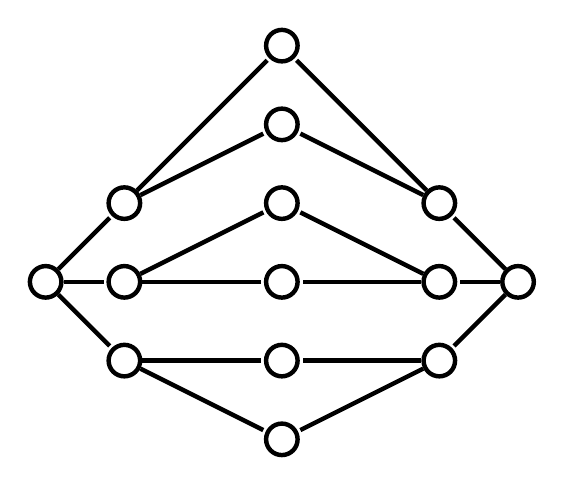
\begin{tikzpicture}[shorten >=1pt, auto, node distance=3cm, ultra thick,main node/.style={circle,draw,minimum size=.4cm,inner sep=0pt]}]%fill=black,
\begin{scope}[every node/.style={font=\sffamily\Large\bfseries}]
\node[main node] (v1) at (0,0) {};
\node[main node] (v2) at (1,1) {};
\node[main node] (v3) at (1,0) {};
\node[main node] (v4) at (1,-1) {};
\node[main node] (v5) at (3,3) {};
\node[main node] (v6) at (3,2) {};
\node[main node] (v7) at (3,1) {};
\node[main node] (v8) at (3,0) {};
\node[main node] (v9) at (3,-1) {};
\node[main node] (vA) at (3,-2) {};
\node[main node] (vB) at (5,0) {};
\node[main node] (vC) at (5,-1) {};
\node[main node] (vD) at (5,1) {};
\node[main node] (vE) at (6,0) {};
\end{scope}
\begin{scope}[every edge/.style={draw=black,ultra thick}]
\draw  (v1) edge node{} (v2);
\draw  (v1) edge node{} (v3);
\draw  (v1) edge node{} (v4);
\draw  (v2) edge node{} (v5);
\draw  (v2) edge node{} (v6);
\draw  (v3) edge node{} (v7);
\draw  (v3) edge node{} (v8);
\draw  (v4) edge node{} (v9);
\draw  (v4) edge node{} (vA);
\draw  (vE) edge node{} (vD);
\draw  (vE) edge node{} (vB);
\draw  (vE) edge node{} (vC);
\draw  (vD) edge node{} (v5);
\draw  (vD) edge node{} (v6);
\draw  (vB) edge node{} (v7);
\draw  (vB) edge node{} (v8);
\draw  (vC) edge node{} (v9);
\draw  (vC) edge node{} (vA);
\end{scope}
\end{tikzpicture}
\caption*{$\mathtt{MAX CUT} = 18$}
\end{figure}
\end{minipage}%
\begin{minipage}{.48\textwidth}
\begin{figure}[H]
\centering
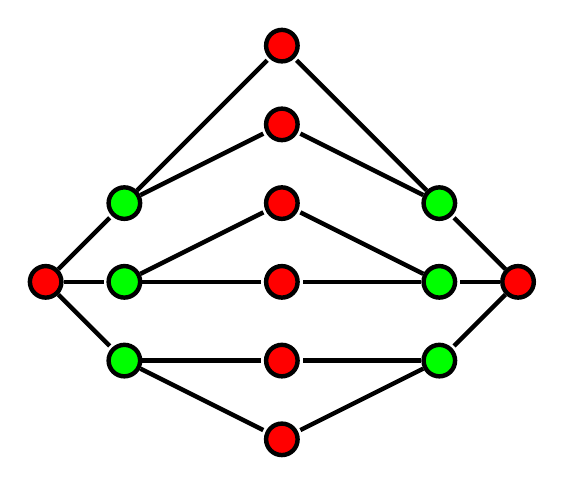
\begin{tikzpicture}[shorten >=1pt, auto, node distance=3cm, ultra thick,main node/.style={circle,draw,minimum size=.4cm,inner sep=0pt]}]%fill=black,
\begin{scope}[every node/.style={font=\sffamily\Large\bfseries}]
\node[main node,fill=red] (v1) at (0,0) {};
\node[main node,fill=green] (v2) at (1,1) {};
\node[main node,fill=green] (v3) at (1,0) {};
\node[main node,fill=green] (v4) at (1,-1) {};
\node[main node,fill=red] (v5) at (3,3) {};
\node[main node,fill=red] (v6) at (3,2) {};
\node[main node,fill=red] (v7) at (3,1) {};
\node[main node,fill=red] (v8) at (3,0) {};
\node[main node,fill=red] (v9) at (3,-1) {};
\node[main node,fill=red] (vA) at (3,-2) {};
\node[main node,fill=green] (vB) at (5,0) {};
\node[main node,fill=green] (vC) at (5,-1) {};
\node[main node,fill=green] (vD) at (5,1) {};
\node[main node,fill=red] (vE) at (6,0) {};
\end{scope}
\begin{scope}[every edge/.style={draw=black,ultra thick}]
\draw  (v1) edge node{} (v2);
\draw  (v1) edge node{} (v3);
\draw  (v1) edge node{} (v4);
\draw  (v2) edge node{} (v5);
\draw  (v2) edge node{} (v6);
\draw  (v3) edge node{} (v7);
\draw  (v3) edge node{} (v8);
\draw  (v4) edge node{} (v9);
\draw  (v4) edge node{} (vA);
\draw  (vE) edge node{} (vD);
\draw  (vE) edge node{} (vB);
\draw  (vE) edge node{} (vC);
\draw  (vD) edge node{} (v5);
\draw  (vD) edge node{} (v6);
\draw  (vB) edge node{} (v7);
\draw  (vB) edge node{} (v8);
\draw  (vC) edge node{} (v9);
\draw  (vC) edge node{} (vA);
\end{scope}
\end{tikzpicture}
\end{figure}
\end{minipage}
Tu mamy graf dwudzielny, a w każdym grafie dwudzielnym $\mathtt{MAX CUT} = E(G)$ czyli w  tym przypadku $\mathtt{MAX CUT} = 18$

\paragraph{A2}
\begin{enumerate}[label=\alph*)]
\item Wyznacz (zdroworozsądkowo) $\mathtt{MAX CUT}$ w grafie $K_{3,3}$.
\item Jakie oszacowanie na $\mathtt{MAX CUT}$ w grafie $K_{3,3}$ daje twierdzenie z wykładu, w którym pojawia się wartość własna laplasjanu?
\end{enumerate}
\begin{minipage}{.45\textwidth}
\begin{figure}[H]
\centering
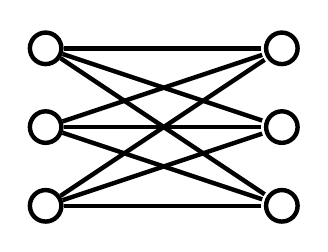
\begin{tikzpicture}[shorten >=1pt, auto, node distance=3cm, ultra thick,main node/.style={circle,draw,minimum size=.4cm,inner sep=0pt]}]%fill=black,
\begin{scope}[every node/.style={font=\sffamily\Large\bfseries}]
\node[main node] (v1) at (0,0) {};%1
\node[main node] (v2) at (0,-1) {};%2
\node[main node] (v3) at (0,-2) {};%3
\node[main node] (v4) at (3,0) {};%4
\node[main node] (v5) at (3,-1) {};%5
\node[main node] (v6) at (3,-2) {};%6
%\node[main node] (v) at (,) {};
\end{scope}
\begin{scope}[every edge/.style={draw=black,ultra thick}]
\draw  (v1) edge node{} (v4);
\draw  (v1) edge node{} (v5);
\draw  (v1) edge node{} (v6);
\draw  (v2) edge node{} (v4);
\draw  (v2) edge node{} (v5);
\draw  (v2) edge node{} (v6);
\draw  (v3) edge node{} (v4);
\draw  (v3) edge node{} (v5);
\draw  (v3) edge node{} (v6);
%\draw  (v) edge node{} (v);
\end{scope}
\end{tikzpicture}
\caption*{$K_{3,3}$}
\end{figure}
\end{minipage}%
\begin{minipage}{.45\textwidth}
\begin{figure}[H]
\centering
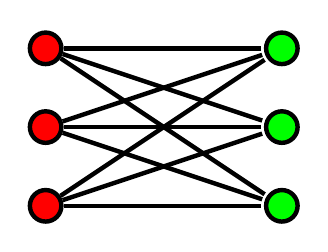
\begin{tikzpicture}[shorten >=1pt, auto, node distance=3cm, ultra thick,main node/.style={circle,draw,minimum size=.4cm,inner sep=0pt]}]%fill=black,
\begin{scope}[every node/.style={font=\sffamily\Large\bfseries}]
\node[main node,fill=red] (v1) at (0,0) {};%1
\node[main node,fill=red] (v2) at (0,-1) {};%2
\node[main node,fill=red] (v3) at (0,-2) {};%3
\node[main node,fill=green] (v4) at (3,0) {};%4
\node[main node,fill=green] (v5) at (3,-1) {};%5
\node[main node,fill=green] (v6) at (3,-2) {};%6
%\node[main node] (v) at (,) {};
\end{scope}
\begin{scope}[every edge/.style={draw=black,ultra thick}]
\draw  (v1) edge node{} (v4);
\draw  (v1) edge node{} (v5);
\draw  (v1) edge node{} (v6);
\draw  (v2) edge node{} (v4);
\draw  (v2) edge node{} (v5);
\draw  (v2) edge node{} (v6);
\draw  (v3) edge node{} (v4);
\draw  (v3) edge node{} (v5);
\draw  (v3) edge node{} (v6);
%\draw  (v) edge node{} (v);
\end{scope}
\end{tikzpicture}
\caption*{$K_{3,3}$}
\end{figure}
\end{minipage}\\
$\mathtt{MAX CUT}=9$


\paragraph{A3} Niech $Pet$ oznacza graf Petersena (pojawił się na liście 3, w zadaniu A3(e)).
\begin{enumerate}[label=\alph*)]
\item Wskaż odpowiedni podział zbioru $V (Pet)$, świadczący o tym, że w grafie istnieje cięcie krawędziowe liczące co najmniej $5$ krawędzi.
\item Wskaż jak największe potrafisz cięcie krawędziowe w grafie Petersena. W tym celu Wskaż odpowiedni podział zbioru wierzchołków.
\end{enumerate}

\begin{figure}[H]
\centering
\begin{tikzpicture}[every node/.style={draw,circle,very thick}]
\graph[clockwise, radius=2cm, n=5,name=A] {subgraph C_n };
\graph[clockwise, radius=1cm, n=5, name=B] { 1/"6", 2/"7", 3/"8", 4/"9", 5/"10"; subgraph I_n };

\foreach \i [evaluate={\j=int(mod(\i+2+4,5)+1)}]
in {1,2,3,4,5}{
	\draw (A \i) -- (B \i);
	\draw (B \j) -- (B \i);
}
\end{tikzpicture}
\caption*{Ten fajny graf Petersena}
\end{figure}
Dla $V=\{2,5,8,9\}$ $\Rightarrow$ $\mathtt{MAX CUT}=12$
\begin{align*}
\mathtt{MAX CUT}&\leq \frac{V(Pet)*\mu _n}{4}\\
\mathtt{MAX CUT}&\leq \frac{10*5}{4}\\
\mathtt{MAX CUT}&\leq 12.5\\
\mathtt{MAX CUT}&\leq 12
\end{align*}

\paragraph{A4} Niech $G$ będzie grafem o $4$ wierzchołkach i $5$ krawędziach. wierzchołki o stopniu trzy mają numery $1$ i $2$, wierzchołki o stopniu dwa mają numery $3$ i $4$.
\begin{enumerate}[label=\alph*)]
\item Narysuj graf $G$.
\item Wyznacz laplasjan tego grafu.
\item Wyznacz liczbę drzew rozpiętych w tym grafie, obliczając minor laplasjanu.
\end{enumerate}
\begin{minipage}{.32\textwidth}
\begin{figure}[H]
%\begin{wrapfigure}{r}{0.3\textwidth}
\centering
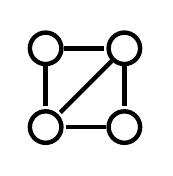
\begin{tikzpicture}[shorten >=1pt, auto, node distance=3cm, ultra thick,main node/.style={circle,draw,minimum size=.4cm,inner sep=0pt]}]%fill=black,
\begin{scope}[every node/.style={font=\sffamily\Large\bfseries}]
\node[main node] (v1) at (0,1) {};%1
\node[main node] (v2) at (1,1) {};%2
\node[main node] (v3) at (1,0) {};%3
\node[main node] (v4) at (0,0) {};%4
\end{scope}
\begin{scope}
\draw  (v1) edge node{} (v2);
\draw  (v1) edge node{} (v4);
\draw  (v2) edge node{} (v3);
\draw  (v2) edge node{} (v4);
\draw  (v3) edge node{} (v4);
%\draw  (v) edge node{} (v);
\end{scope}
\end{tikzpicture}
\caption*{Graf $G$.}
%\end{wrapfigure}
\end{figure}
\end{minipage}%
\begin{minipage}{.32\textwidth}
$$L=\begin{bmatrix}
2&-1&0&-1\\
-1&3&-1&-1\\
0&-1&2&-1\\
-1&-1&-1&3
\end{bmatrix}$$
\end{minipage}
\begin{align*}
\det (L)=\begin{vmatrix}
2&-1&0&-1\\
-1&3&-1&-1\\
0&-1&2&-1\\
-1&-1&-1&3
\end{vmatrix}=\left|
\begin{array}{ccc>{\columncolor{red!20}}c}
2&-1&0&-1\\
-1&3&-1&-1\\
0&-1&2&-1\\\rowcolor{red!20}
-1&-1&-1&3
\end{array}
\right| = \begin{vmatrix}
2&-1&0\\-1&3&-1\\0&-1&2
\end{vmatrix} = 12-2-2=8
\end{align*}

\paragraph{A5} Demon zastąpił niektóre liczby z podanego laplasjanu grafu G znakami zapytania.
\begin{enumerate}[label=\alph*)]
\item Uzupełnij laplasjan.
\item Wyznacz liczbę drzew rozpiętych w tym grafie, obliczając minor laplasjanu.
\item Narysuj graf $G$.
\end{enumerate}
\begin{minipage}{.3\textwidth}
$$\begin{bmatrix}
3&?&-1&-1\\
-1&?&-1&?\\
-1&?&?&-1\\
?&?&-1&2
\end{bmatrix}$$
Macierz demona
\end{minipage}%
\begin{minipage}{.3\textwidth}
$$\begin{bmatrix}
3&-1&-1&-1\\
-1&2&-1&0\\
-1&-1&3&-1\\
-1&0&-1&2
\end{bmatrix}$$
Macierz ,,Naprawiona''
\end{minipage}%
\begin{minipage}{.3\textwidth}
\begin{figure}[H]
%\begin{wrapfigure}{r}{0.3\textwidth}
\centering
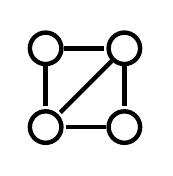
\begin{tikzpicture}[shorten >=1pt, auto, node distance=3cm, ultra thick,main node/.style={circle,draw,minimum size=.4cm,inner sep=0pt]}]%fill=black,
\begin{scope}[every node/.style={font=\sffamily\Large\bfseries}]
\node[main node] (v1) at (0,1) {};%1
\node[main node] (v2) at (1,1) {};%2
\node[main node] (v3) at (1,0) {};%3
\node[main node] (v4) at (0,0) {};%4
\end{scope}
\begin{scope}
\draw  (v1) edge node{} (v2);
\draw  (v1) edge node{} (v4);
\draw  (v2) edge node{} (v3);
\draw  (v2) edge node{} (v4);
\draw  (v3) edge node{} (v4);
%\draw  (v) edge node{} (v);
\end{scope}
\end{tikzpicture}
\caption*{Graf $G$.}
%\end{wrapfigure}
\end{figure}
\end{minipage}
$$\tau (G) = \frac{1}{4}4*4*2=8$$

\paragraph{A6}
\begin{enumerate}[label=\alph*)]
\item Jakiemu parametrowi grafu $G$ jest równy Ślad jego laplasjanu?

Ślad Laplasjanu -suma przekątnej- zawiera sumę stopni wierzchołków grafu która jest równa podwojonej liczbie krawędzi: $$\sum _{i=1}^n\deg (i)=2E(G)$$ 
\item Jakiemu parametrowi grafu $G$ jest równa suma wartości własnych jego laplasjanu?

Suma wartości własnych Laplasjanu $L$ jest równa:
$$\mathsf{Tr}(L)=\sum _{i=1}^n \mu _i=2E(G)$$
\item Znajdź liczbę drzew rozpiętych w grafie $G$ o $5$ wierzchołkach i sześciu krawędziach, wiedząc, że cztery z pięciu wartości własnych jego laplasjanu to: $0, 2, 2$ i $3$.
$$G=(V,E)\ \ V(G)=5\ \ E(G)=6$$
\begin{align*}
\mu _1=0,\ \mu _2=2,\ \mu _3=2,\ \mu _4=3,\ \mu _5=?\\
0+2+2+3+x=12\ \Rightarrow \ x=5\\
\tau (G)=\frac{1}{5}\mu _5*\mu _4*\mu_3*\mu_2 = 12
\end{align*}
\end{enumerate}

\paragraph{A7} Wszystkie wartości własne macierzy przyległości pewnego grafu $3$-regularnego $G$ to: $3, 1, 1, 1, 1, 1, -2,-2,-2,-2$.
\begin{enumerate}[label=\alph*)]
\item Wyznacz spektrum laplasjanu tego grafu.

Posługując się twierdzeniem: $\mu _i=d-\lambda _i,\, i=1,2,..,n$ i dla $d=3$
$$\begin{array}{l|cccccccccc}
\lambda & 3& 1& 1& 1& 1& 1& -2&-2&-2&-2\\\hline
\mu & 0&2&2&2&2&2&5&5&5&5
\end{array}$$
\item Ile jest wszystkich drzew rozpiętych w $G$?

\begin{align*}
\tau (G)&=\frac{1}{n}\mu_n \mu_{n-1}...\mu _2\\
\tau (G)&=\frac{1}{10}2^5*5^4=2000
\end{align*}
\end{enumerate}
 
\paragraph{A8} Niech $G$ będzie ścieżką o trzech wierzchołkach. Znajdź wszystkie wartości własne jej laplasjanu, Rozwiązując równanie $\bar{\bar{L}}\bar{x} = \mu \bar{x}$ lub równanie charakterystyczne $\det(\bar{\bar{L}} - \mu \bar{\bar{L}}) = 0$.

\begin{minipage}{.3\textwidth}
\begin{figure}[H]
%\begin{wrapfigure}{r}{0.3\textwidth}
\centering
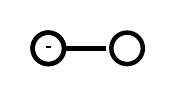
\begin{tikzpicture}[shorten >=1pt, auto, node distance=3cm, ultra thick,main node/.style={circle,draw,minimum size=.4cm,inner sep=0pt]}]%fill=black,
\begin{scope}[every node/.style={font=\sffamily\Large\bfseries}]
\node[main node] (v1) at (1,0) {};%1
\node[main node] (v2) at (1,0) {};%2
\node[main node] (v3) at (2,0) {};%3
\end{scope}
\begin{scope}
\draw  (v1) edge node{} (v2);
\draw  (v2) edge node{} (v3);
%\draw  (v) edge node{} (v);
\end{scope}
\end{tikzpicture}
\caption*{Graf $G$.}
%\end{wrapfigure}
\end{figure}
\end{minipage}%
\begin{minipage}{.3\textwidth}
$$A=\begin{bmatrix}
0&1&0\\1&0&1\\0&0&1
\end{bmatrix}$$
\end{minipage}%
\begin{minipage}{.3\textwidth}
$$L=\begin{bmatrix}
1&-1&0\\-1&2&-1\\0&-1&1
\end{bmatrix}$$
\end{minipage}
\begin{enumerate}[label=\Roman*)]
\item \begin{align*}
\det (L-\mu I)&= \det \left(\begin{bmatrix}
1&-1&0\\-1&2&-1\\0&-1&1
\end{bmatrix}-\mu \begin{bmatrix}
1&0&0\\0&1&0\\0&0&1
\end{bmatrix}\right)=\\
&=\begin{vmatrix}
1-\mu &-1    &0\\
-1    &2-\mu &-1\\
0     &-1    &1-\mu
\end{vmatrix} =\\ 
&= (1-\mu )(2-\mu)(1-\mu )-(-1)(-1)(1-\mu )-(1-\mu )(-1)(-1)=\\
&=-\mu ^3+4\mu ^2-3\mu =\mu (1-\mu )(\mu -3)
\end{align*}
$$\mu_1 = 0,\ \mu _2 = 1,\ \mu _3 = 3$$
\end{enumerate}

\paragraph{A9} oceń poprawność każdego z poniższych zdań. W każdym przypadku poprzyj odpowiedź, w zależności od potrzeby, uzasadnieniem ogólnym, przykładem lub kontrprzykładem.
\begin{enumerate}[label=\alph*)]
\item Jeżeli na przekątnej laplasjanu grafu $G$ są same piątki, to pięć jest wartością własna macierzy przyległości grafu $G$.

\textbf{TAK} wynika, top z faktu, że $G$ jest $5$-regularny (przekątna Laplasjanu oznacza stopnie wierzchołków) a w grafach regularnych wartością własną macierzy jest jej stopień. 
\item Istnieje graf, dla którego spektrum laplasjanu wygląda tak: $5,5,3,3,0,-1,-1$.

\textbf{NEIN} Wartości własne Laplasjanu są NIE ujemne.
\item Istnieje graf, dla którego spektrum laplasjanu wygląda tak: $5,5,3,3,1,1,1,1$.

\textbf{NO} W spektrum Laplasjanu musi być (przynajmniej) jedno $0$
\item Jeżeli w spektrum laplasjanu grafu jest więcej niż jedno zero, to graf ten nie ma drzew rozpiętych.

\textbf{TAK} wzorując się na twierdzeniu Kirchoffa: $$\tau (G)=\frac{1}{n}\mu _n\mu_{n-1}...\mu _2$$
\item Jeżeli graf jest Spójny, to w spektrum laplasjanu jest dokładnie jedno zero.

\textbf{TAK} każdy graf spójny ma drzewo rozpięte, a gdyby miałby więcej niż jedno zero to twierdzenie podane wyżej nie miało by ,,mocy''
\item Jeżeli spektrum laplasjanu grafu $G$ wygląda tak: $4,4,4,4,4,4,0,0$, to $E(G) = 12$.

\begin{align*}
\mathsf{Tr}(A)=\sum _{i=1}^n \lambda _i = 0\\
\mathsf{Tr}(L)=\sum _{i=1}^n \mu _i = 2E(G)\\
\mathsf{Tr}(L)=4+4+4+4+4+4+0+0=24 = 2E(G)
\end{align*}
\textbf{SI!}
\item jedną z wartości własnych laplasjanu każdego $5$– regularnego grafu dwudzielnego jest $10$.

\begin{align*}
\lambda _1 = 5, \underbrace{...}_{n-2} \lambda _n = -5\\
\mu _i = d-\lambda _i\\
\mu _1 = 5-5 = 0\\
\mu _n = 5--5=10
\end{align*}
\textbf{OUI!}
\end{enumerate}

\subsection{Zadania Domowe B}
\paragraph{B1} Niech $G$ będzie ,,trójkątem z ogonkiem”, tzn. jedynym grafem o czterech wierzchołkach z ciągiem stopni $(3, 2, 2, 1)$. Wiadomo, że trzy z czterech wartości własnych laplasjanu tego grafu wynoszą 0, 3 i 4. Znajdź czwartą wartość własną i Rozwiązując odpowiedni układ równań Znajdź odpowiadający jej wektor własny.

\paragraph{B2} Pięć z sześciu wartości własnych laplasjanu cyklu $C_6$ to: 4, 3, 1, 1, 0. Znajdź szóstą wartość własną i podaj liczbę drzew rozpiętych w $C_6$.

\paragraph{B3} Graf $G$ ma 6 wierzchołków i 9 krawędzi, a pięć z sześciu wartości własnych jego laplasjanu to: 0, 2, 2, 4 i 4. Znajdź górne oszacowanie na MAXCUT w tym grafie.

\paragraph{B4}
\begin{enumerate}[label=\alph*)]
\item Jakie liczby całkowite na pewno są wartościami własnymi laplasjanu dwudzielnego grafu 8-regularnego?
\item Jakie liczby całkowite na pewno nie są wartościami własnymi laplasjanu dwudzielnego grafu 8-regularnego?
\item G jest dwudzielnym grafem 8-regularnym o 32 wierzchołkach. Wyznacz wartości własne laplasjanu grafu G (wraz z krotnościami), wiedząc, że ma on 3 różne wartości własne.
\end{enumerate}

\paragraph{B5} Oto laplasjan $L$ pewnego grafu $G$, o którym wiadomo, że największej wartości własnej macierzy $L$ odpowiada wektor $(1, 1, 1, 1, 1, 1, -1, -1, -1, -1, -1, -1)$. Oszacuj z góry jak najlepiej potrafisz liczbę krawędzi w największym cięciu grafu $G$.
\begin{figure}[H]
\centering
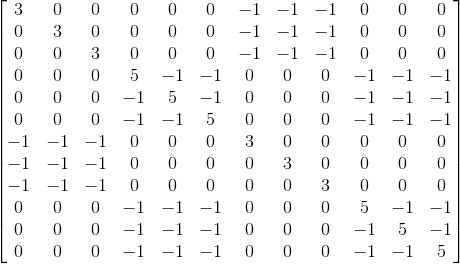
\includegraphics[width=.9\textwidth]{img/5_B5}
\end{figure}
\todo[inline,color=red]{ZADANIE ZAPYTAĆ!}

\paragraph{B6} Niech G będzie grafem o ciągu stopni (3, 3, 2, 2), tzn. G jest cyklem o długości 4 z jedną przekątną.
\begin{enumerate}[label=\alph*)]
\item Znajdź, nie Korzystając z żadnych wzorów, liczbę t(G) drzew rozpiętych grafu G.
\item Znajdź t(G) obliczając minor laplasjanu G.
\item Dobra wróżka powiedziała, że wektorami własnymi laplasjanu grafu G są: (-2, 0, 1, 1), (-1, 1, 0, 0), (0, 0, -1, 1), (1, 1, 1, 1), gdzie pierwsze dwie współrzędne odpowiadają wierzchołkom o stopniu trzy. Znajdź wszystkie wartości własne laplasjanu.
\item Znajdź t(G) Korzystając z własności własnych znalezionych w poprzednim podpunkcie.
\end{enumerate}

\paragraph{B7} Załóżmy, że znamy spektrum i bazę wektorów własnych dla laplasjanu każdej składowej niespójnego grafu G. Jak wyznaczyć szybko spektrum i bazę wektorów własnych dla laplasjanu grafu G?

\paragraph{B8} Wyznacz spektrum i bazę wektorów własnych laplasjanu grafu złożonego z wierzchołkowo rozłącznych K3 i C4 oraz z wierzchołka izolowanego.

\paragraph{B9} Dane jest spektrum laplasjanu pewnego 2–regularnego grafu G: 3, 3, 3, 3, 0, 0. Narysuj graf G (i uzasadnij, że z dokładnością do izomorfizmu nie ma innych).

\paragraph{B10} Spektrum laplasjanu pewnego 3–regularnego grafu G wygląda tak: 0, 2, 2, 2, 2, 2, 5, 5, 5, 5. Ile cykli o długości 3 zawiera G?

\paragraph{B11} oceń poprawność każdego z poniższych zdań. W każdym przypadku poprzyj odpowiedź, w zależności od potrzeb, uzasadnieniem ogólnym, przykładem lub kontrprzykładem. W wszystkich podpunktach wartości własne dotyczą macierzy przyległości rozważanego grafu,
\begin{enumerate}[label=\alph*)]
\item  Istnieje niepusty graf, dla którego wszystkie wartości własne laplasjanu są takie same.
\item  Istnieje graf 3–regularny, dla którego spektrum laplasjanu wygląda tak: 5, 5, 5, 3, 3, 3, 3, 0, 0.
\item  Jeżeli największa wartość własna laplasjanu grafu jest mniejsza od 8, a w grafie istnieje cięcie liczące 100 krawędzi, to graf ten ma przynajmniej 50 wierzchłków.
\item  Jeżeli laplasjan grafu G jest macierzą $10 \times 10$ i ma same 5 na przekątnej, to G jest nieplanarny.
\end{enumerate}

\paragraph{B12} Macierz przyległości A pewnego 3–regularnego grafu na 10 wierzchołkach spełnia równanie: A2 + A - 2I - J = 0. Wyznacz wszystkie wartości własne laplasjanu L i Znajdź liczbę drzew rozpiętych dla tego grafu.

\todo[inline,color=red]{ZADANIE ZAPYTAĆ!}
\paragraph{B13} Załóżmy, że graf G o 50 wierzchołkach jest 7–regularny. Ponadto macierz przyległości A tego grafu spełnia równanie: A2 = J - A + 6I,
J oznacza macierz złożoną z samych jedynek, a I jest macierzą jednostkową. Wyciągnij jak najwięcej informacji o grafie G, dotyczących:
\begin{enumerate}[label=\alph*)]
\item dwudzielności,
\item planarności,
\item liczby cykli długości trzy, jakie G zawiera,
\item liczby drzew rozpiętych,
\item oszacowania MAXCUT z dołu i z góry.
\end{enumerate}
Wskazówka: Na niektóre z powyższych pytań można odpowiedzieć, nie przejmując się podanym równaniem.
\todo[inline,color=red]{ZADANIE ZAPYTAĆ!}

\subsection{Zadania}
\paragraph{Zad.1} Uzasadnij, że regularny graf $G$ jest Spójny wtedy i tylko wtedy, gdy największa wartość własna jego macierzy przyległości jest $1$-krotna. Uwaga: Niestety nie jest to prawdą dla grafów nieregularnych.

\textbf{Odpowiedź: } $G\rightarrow $ $d$-regularny\\
Cel: $G\rightarrow$ spójny $\Leftrightarrow$ największa własność własna $A$ jest jednokrotna
\begin{itemize}
\item[$\Rightarrow$]
\begin{enumerate}
\item $G$ jest spójny,
\item $G$ ma drzewo rozpięte
\item $\tau (G)=\frac{1}{n}\mu_2\mu_3...\mu_n>0$
\item $\mu_2\mu_3...\mu_n>0$
\item $G$ jest $d$-regularny
\item $d-\lambda _2, d-\lambda _3...d-\lambda _n>0$
\item $\lambda _2 < d, \lambda _3<d...\lambda _n<d$
\end{enumerate}
$d$ jest wartością własną, bo $G$ jest regularny, więc $d$ jest jednokrotną wartością własną $A$.
\item[$\Leftarrow$] Ogólnie dowód jak wyżej tylko w ,,odwrotną stronę''
\end{itemize}
\paragraph{Zad.2} Dobra wróżka zdradziła, że wszystkie wartości własne macierzy przyległości grafu Petersena $Pet$ należą do zbioru $\{-2, 1, 3\}$.
\begin{enumerate}[label=\alph*)]
\item Wyznacz spektrum laplasjanu dla $Pet$.
\item Oblicz dla tego grafu liczbę wszystkich drzew rozpiętych.
\item Wyznacz $\mathsf{MAXCUT}$.
\end{enumerate}

\paragraph{Zad.3} Znajdź liczbę drzew rozpiętych w grafie $K_{2,3}$, licząc minor laplasjanu. Chętni mogą policzyć je kombinatorycznie.

\paragraph{Zad.4} Dobra wróżka zdradziła nam pierwszy wiersz laplasjanu $L$ pewnego grafu na $6$ wierzchołkach oraz $6$ liniowo niezależnych wektorów własnych macierzy $L$.
\begin{enumerate}[label=\alph*)]
\item Wyznacz liczbę drzew rozpiętych w rozważanym grafie.
\item Oszacuj z góry i z dołu liczbę krawędzi w największym cięciu tego grafu.
\end{enumerate}
Pierwszy wiersz macierzy $L:$
$$[3,-1,0,-1,0,-1]$$
wektory własne:
$$\begin{bmatrix}
2\\-2\\-1\\1\\-1\\1
\end{bmatrix},\ \begin{bmatrix}
1\\0\\1\\0\\-2\\0
\end{bmatrix},\ \begin{bmatrix}
1\\1\\1\\1\\1\\1
\end{bmatrix},\ \begin{bmatrix}
-1\\1\\-1\\1\\-1\\1
\end{bmatrix},\ \begin{bmatrix}
3\\0\\-3\\0\\0\\0
\end{bmatrix},\ \begin{bmatrix}
-1\\0\\0\\0\\1\\0
\end{bmatrix}$$


